% =====================================================================
% folha_controle.tex -- Adaptacao para LaTeX da "Folha de Controle de
% Documentos Complexos" real do RMB (extraida de
% RMBN0000LNG7240RA001BCap1_4.docx), paginas 1-2.
% =====================================================================
\newcommand{\folharodape}{%
  \vspace{2pt}
  \noindent\rule{\textwidth}{0.4pt}\\[1pt]
  {\footnotesize\'E proibida a duplica\c{c}\~ao ou reprodu\c{c}\~ao deste volume ou de parte do mesmo, sob quaisquer meios, sem autoriza\c{c}\~ao expressa da CNEN\hfill\thepage}%
}

\newcommand{\folhacabecalho}[1]{%
\begin{tabular}{|>{\centering\arraybackslash}p{0.20\textwidth}|>{\centering\arraybackslash}p{0.62\textwidth}|}
\hline
\raisebox{-0.3\height}{\sffamily\bfseries\large CNEN RMB} &
\sffamily\bfseries COMISS\~AO NACIONAL DE ENERGIA NUCLEAR\newline
\sffamily\small\mdseries DIRETORIA DE PESQUISA E DESENVOLVIMENTO\newline
\sffamily\small\mdseries REATOR MULTIPROP\'OSITO BRASILEIRO \\
\hline
\multicolumn{2}{|>{\centering\arraybackslash}p{0.84\textwidth}|}{\rule{0pt}{14pt}\sffamily\bfseries #1}\\[2pt]
\hline
\end{tabular}%
}

% ---------------------------------------------------------------------
% Pagina 1 -- reproduzida como figura a partir do proprio DOCX real
% (RMBN0000LNG7240RA001BCap1_4.docx, pagina 1), a pedido do requerente:
% a recriacao em tabelas LaTeX nao ficou esteticamente satisfatoria,
% entao a pagina passa a ser "colada" como imagem, fiel ao original.
% ---------------------------------------------------------------------
\thispagestyle{empty}
\noindent\centering
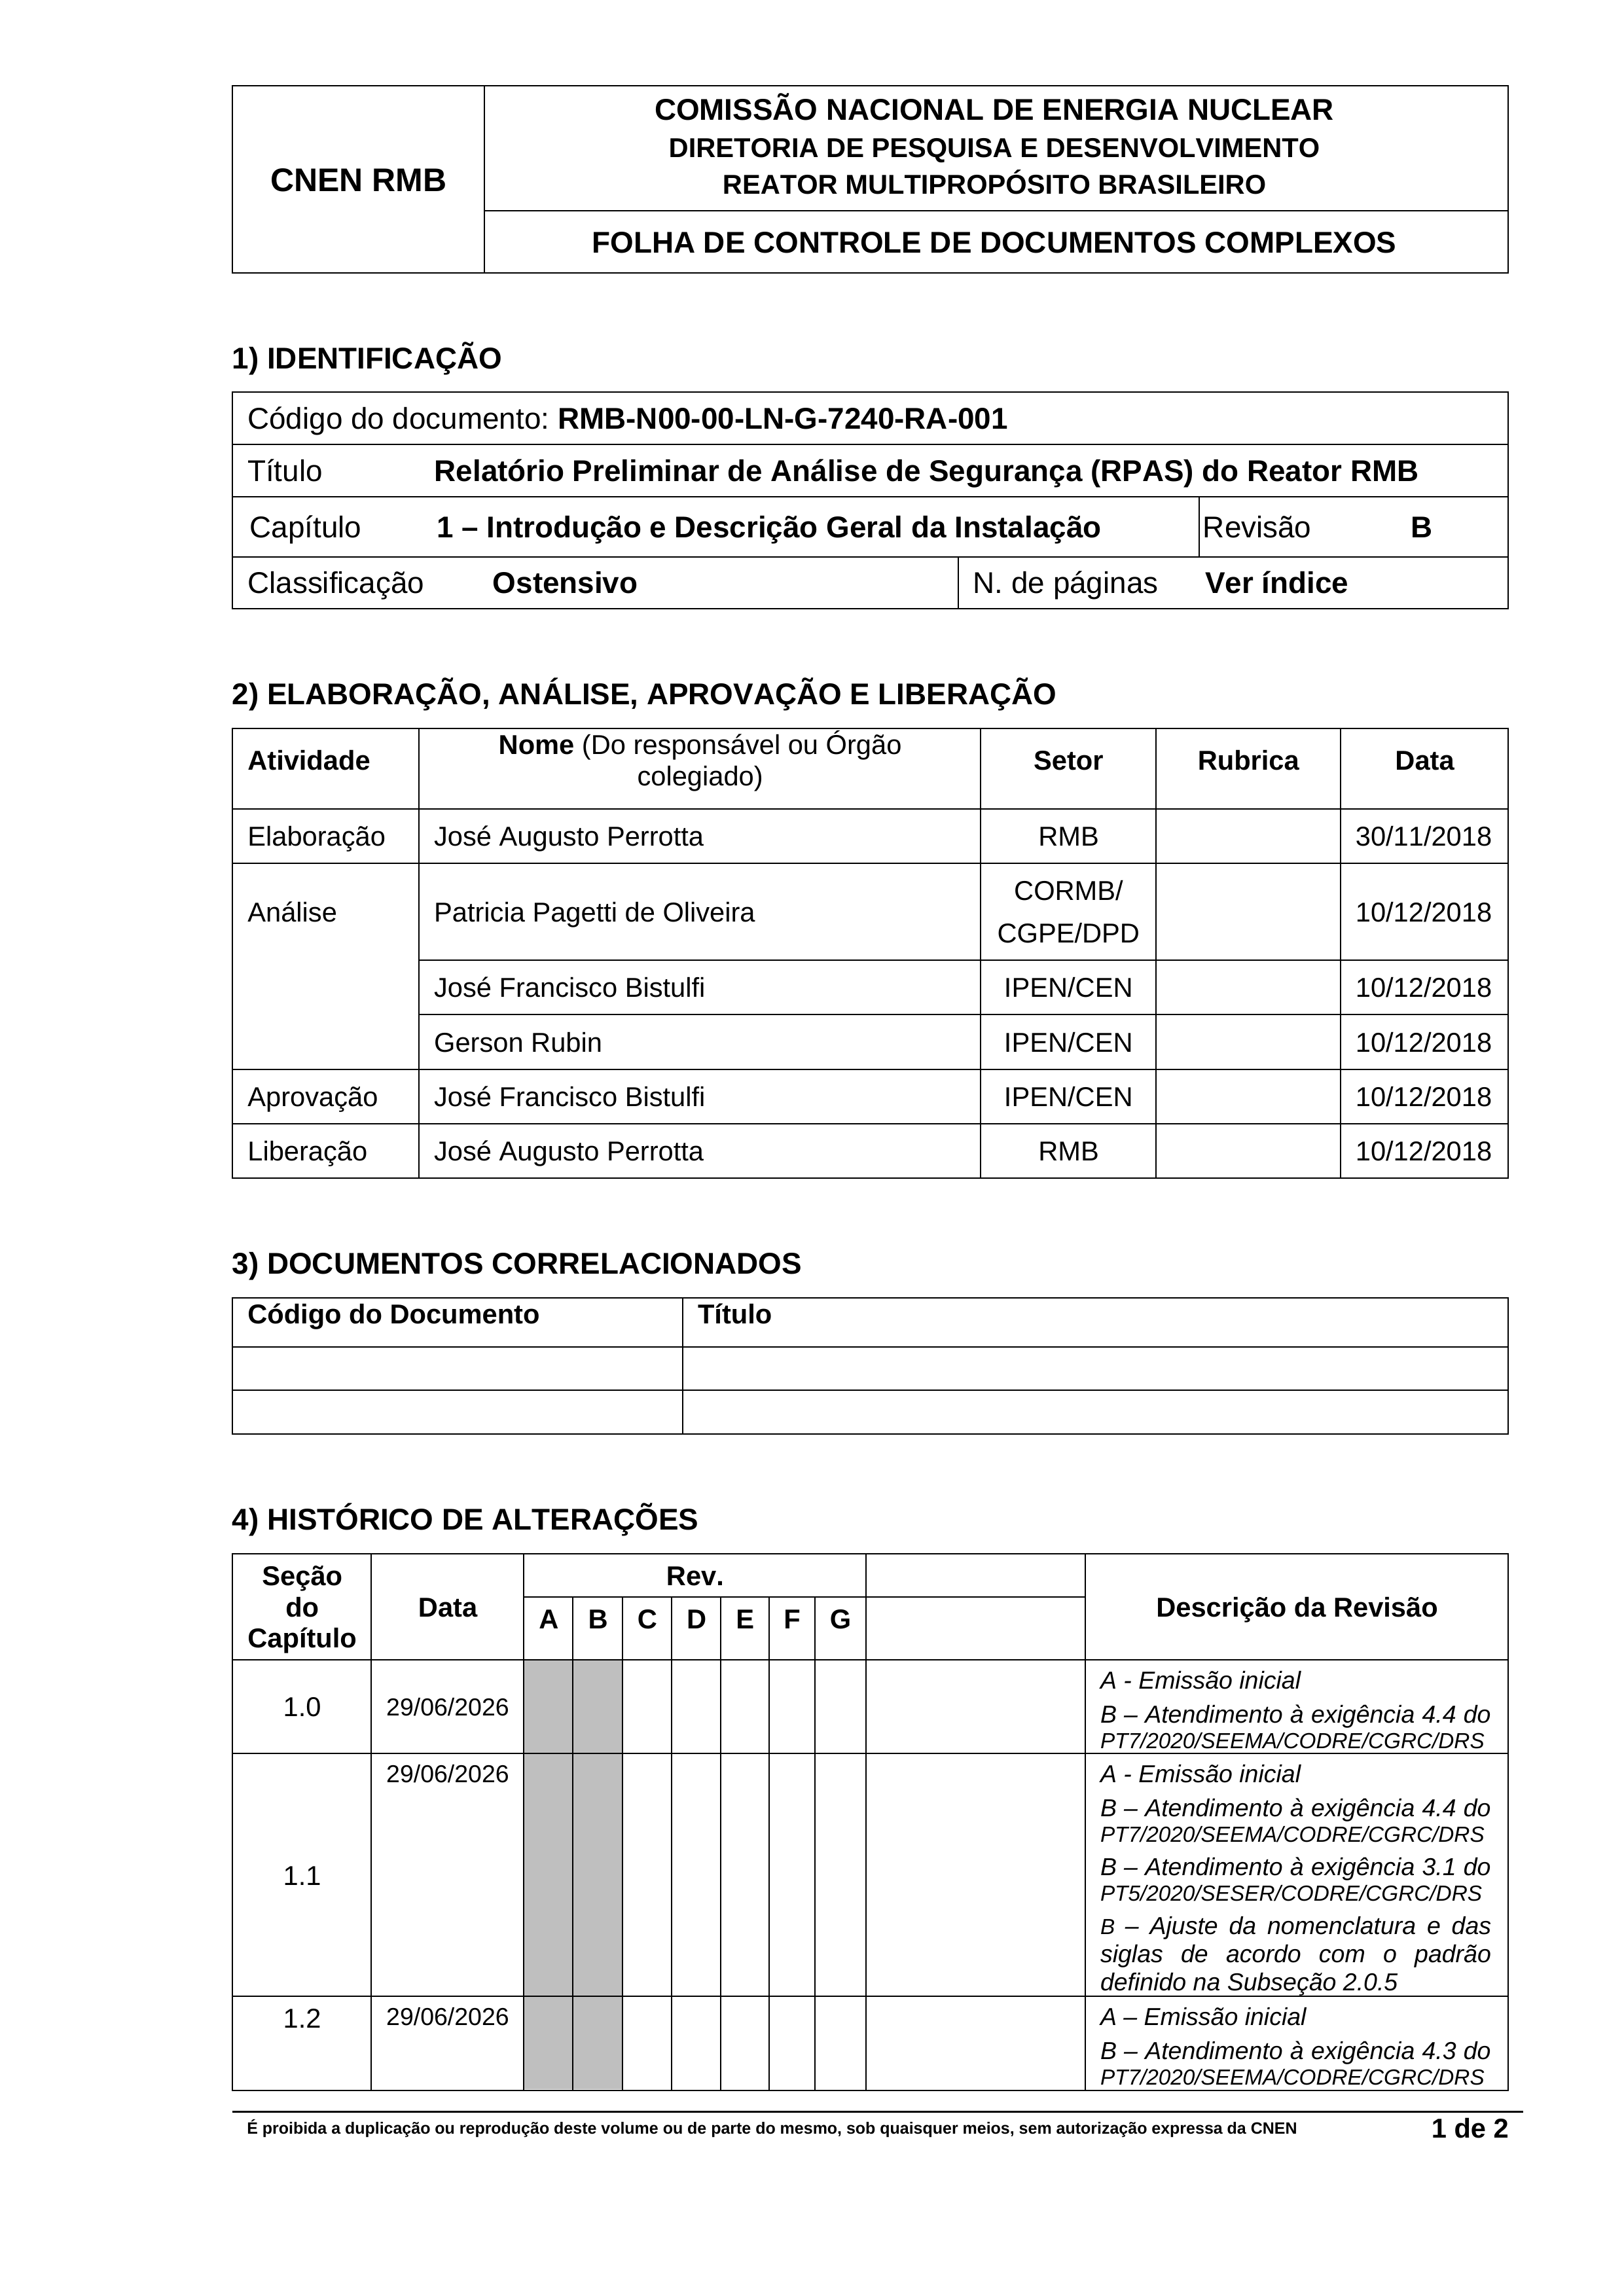
\includegraphics[width=\textwidth,height=0.97\textheight,keepaspectratio]{figures/folha_controle_pagina1.png}
\par
\clearpage

% =====================================================================
% Pagina 2 -- Historico de alteracoes (mantida em LaTeX)
% =====================================================================
\newgeometry{top=1.6cm,bottom=2.5cm,left=3.0cm,right=2.3cm}
\thispagestyle{empty}
\setlength{\parindent}{0pt}
\singlespacing
\renewcommand{\arraystretch}{0.72}
\setlength{\tabcolsep}{4pt}

\folhacabecalho{FOLHA DE CONTROLE DE DOCUMENTOS}

\vspace{5pt}

{\sffamily\bfseries 4) HIST\'ORICO DE ALTERA\c{C}\~OES}

\vspace{2pt}
\begin{longtable}{|>{\footnotesize\centering\arraybackslash}p{0.08\textwidth}|>{\footnotesize\centering\arraybackslash}p{0.135\textwidth}|>{\footnotesize\centering\arraybackslash}p{0.025\textwidth}|>{\footnotesize\centering\arraybackslash}p{0.025\textwidth}|>{\footnotesize\centering\arraybackslash}p{0.025\textwidth}|>{\footnotesize\raggedright\arraybackslash}p{0.52\textwidth}|}
\hline
\textbf{Se\c{c}\~ao} & \textbf{Data} & \textbf{A} & \textbf{B} & \textbf{C} & \textbf{Descri\c{c}\~ao da Revis\~ao} \\
\hline
\endfirsthead
\hline
\textbf{Se\c{c}\~ao} & \textbf{Data} & \textbf{A} & \textbf{B} & \textbf{C} & \textbf{Descri\c{c}\~ao da Revis\~ao} \\
\hline
\endhead
\hline
\endfoot

1.0 & 29/06/2026 & \cellcolor{nutablehead} & \cellcolor{nutablehead} & &
{\footnotesize\emph{A -- Emiss\~ao inicial}\newline
\emph{B -- Atendimento \`a exig\^encia 4.4 do PT7/2020/SEEMA/CODRE/CGRC/DRS}} \\
\hline
1.1 & 29/06/2026 & \cellcolor{nutablehead} & \cellcolor{nutablehead} & &
{\footnotesize\emph{A -- Emiss\~ao inicial}\newline
\emph{B -- Atendimento \`a exig\^encia 4.4 do PT7/2020/SEEMA/CODRE/CGRC/DRS}\newline
\emph{B -- Atendimento \`a exig\^encia 3.1 do PT5/2020/SESER/CODRE/CGRC/DRS}\newline
\emph{B -- Ajuste da nomenclatura e das siglas conforme a Subse\c{c}\~ao 2.0.5}} \\
\hline
1.2 & 29/06/2026 & \cellcolor{nutablehead} & \cellcolor{nutablehead} & &
{\footnotesize\emph{A -- Emiss\~ao inicial}\newline
\emph{B -- Atendimento \`as exig\^encias 4.3 e 4.4 do PT7/2020/SEEMA/CODRE/CGRC/DRS}\newline
\emph{B -- Ajuste da nomenclatura e das siglas conforme a Subse\c{c}\~ao 2.0.5}\newline
\emph{B -- Inclus\~ao de novas cita\c{c}\~oes a outros Cap\'itulos, se\c{c}\~oes, subse\c{c}\~oes e itens do RPAS}} \\
\hline
1.3 & 29/06/2026 & \cellcolor{nutablehead} & \cellcolor{nutablehead} & &
{\footnotesize\emph{A -- Emiss\~ao inicial}\newline
\emph{B -- Atendimento \`as exig\^encias 4.2 e 4.4 do PT7/2020/SEEMA/CODRE/CGRC/DRS e 4.1 do PT35/2019/SEASE/CODRE/CGRC/DRS}\newline
\emph{B -- Ajuste da nomenclatura e das siglas conforme a Subse\c{c}\~ao 2.0.5}\newline
\emph{B -- Inclus\~ao de novas cita\c{c}\~oes a outros Cap\'itulos, se\c{c}\~oes, subse\c{c}\~oes e itens do RPAS}} \\
\hline
1.4 & 29/06/2026 & \cellcolor{nutablehead} & \cellcolor{nutablehead} & &
{\footnotesize\emph{A -- Emiss\~ao inicial}\newline
\emph{B -- Ajuste da nomenclatura e das siglas conforme a Subse\c{c}\~ao 2.0.5 e ajuste de cita\c{c}\~ao \`a outra se\c{c}\~ao do Cap\'itulo}} \\
\hline
1.5 & 29/06/2026 & \cellcolor{nutablehead} & \cellcolor{nutablehead} & &
{\footnotesize\emph{A -- Emiss\~ao inicial}\newline
\emph{B -- Atendimento \`a exig\^encia 4.1 do PT7/2020/SEEMA/CODRE/CGRC/DRS}} \\
\hline
1.6 & 10/12/2018 & \cellcolor{nutablehead} & & &
{\footnotesize\emph{A -- Emiss\~ao inicial}} \\
\hline
1.7 & 10/12/2018 & \cellcolor{nutablehead} & & &
{\footnotesize\emph{A -- Emiss\~ao inicial}} \\
\hline
\end{longtable}

\folharodape
\restoregeometry
